\documentclass[10pt,twocolumn,letterpaper]{article}
\usepackage{microtype}
\usepackage{booktabs}
\usepackage{hyperref}
\usepackage{graphicx}
\usepackage{amsmath,amssymb}
\usepackage{cleveref}
\usepackage{textcomp}
\usepackage{xcolor}
\usepackage{siunitx}
\raggedbottom

\title{An Autonomous Evaluation Framework for Quantitative Robustness, Faithful Explainability, and Failure-Mode Auditing in Vision Models}
\author{William Steve Rodriguez Villamizar (wisrovi rodriguez)\\AI Leader \& Solutions Architect\\wisrovi-suit (https://github.com/wisrovi/w-cli)}
\date{}

\begin{document}
\maketitle

\section{Abstract \& Keywords}
\textbf{Abstract:} Object detectors in production are certified on a single number---in-distribution mAP---which says nothing about adversarial vulnerability, sensitivity to sensor corruptions, the faithfulness of their explanations, or the failure modes that dominate in the field. We present an autonomous evaluation framework that quantifies all four dimensions in a single post-training pass and turns them into objective, thresholded risk flags that gate deployment. The framework composes six states: (1) multi-attack adversarial testing using FGSM, PGD-20, and Carlini-Wagner (C\&W) $L_2$ attacks across five perturbation magnitudes; (2) corruption robustness across five severity levels of five corruption families (Gaussian blur, Gaussian noise, JPEG compression, motion blur, and impulse noise); (3) MC Dropout uncertainty decomposition into epistemic and aleatoric variance over 20 forward passes paired with Expected Calibration Error (ECE) monitoring; (4) quantitative XAI fidelity via Deletion and Insertion AUC with Grad-CAM++ and Eigen-CAM; (5) a hard-negative mining audit that clusters 450 field failures into background confusion (49.3\% $\pm$ 1.8\%), localization (20.0\% $\pm$ 1.1\%), missed detection (16.9\% $\pm$ 0.9\%), and similarity/other (13.8\% $\pm$ 0.8\%); and (6) an LLM reporting state with a deterministic fallback that guarantees a valid report in 0.03\,ms median even when the model call fails. Across the six states, only the LLM path and the uncertainty sampling involve stochastic draws; every analytic result is a deterministic function of the weights and inputs, making the audit reproducible bit-for-bit. We report that adversarial attacks degrade up to 82.5\% of detections under PGD-20 at $\epsilon=0.20$, and corruption severity 5 cuts confidence by more than 40\%. Grad-CAM++ and Eigen-CAM reduce Deletion AUC to 0.199 and 0.162 (random baseline 0.471) while retaining Insertion AUC of 0.815 and 0.860. The failure audit shows that background confusion dominates field error. Each dimension maps to an objective risk threshold justified via sensitivity sweeps, and a deployment gate rejects the model when any dimension breaches its bound.

\textbf{Keywords:} Robustness, Adversarial Attacks, FGSM, PGD, Carlini-Wagner, MC Dropout, ECE Calibration, Grad-CAM++, Eigen-CAM, Deletion AUC, Failure-Mode Auditing, MLOps, Object Detection.


\section{Author Information}
This research was conceptualized and developed by William Steve Rodriguez Villamizar (wisrovi rodriguez), AI Leader \& Solutions Architect for the wisrovi-suit ecosystem (https://github.com/wisrovi/w-cli). Contact: wisrovi.rodriguez@gmail.com.

\section{Introduction}
Certifying that a computer vision model is ``safe to deploy'' with a single accuracy number is like certifying an aircraft with a top-speed figure. The mAP of a YOLO detector on its held-out set encodes nothing about the perturbations that will actually hit it in the field: adversarial input crafted by an attacker, sensor blur and compression on an aging camera, predictions the model is confidently wrong about, explanations that highlight the wrong pixels, and failure modes that cluster in specific scene conditions.

Each of these dimensions has a mature research community. Adversarial testing suites assess model robustness against perturbations like FGSM~\cite{goodfellow2015fgsm}, iterative projected gradient descent (PGD)~\cite{madry2018towards}, optimization-based attacks like Carlini-Wagner (C\&W)~\cite{carlini2017towards}, and ensemble benchmarks like AutoAttack~\cite{croce2020reliable}, defining a complex space of vulnerabilities~\cite{silva2020opportunities}. Corruption benchmarks measure degradation under realistic sensor noise~\cite{hendrycks2019benchmarking}; MC Dropout decomposes predictive uncertainty into its epistemic and aleatoric components~\cite{gal2016dropout,kendall2017uncertainties}; Deletion and Insertion AUC measure whether saliency maps faithfully identify the pixels driving a prediction~\cite{petsiuk2018rise,chattopadhay2018gradcam,selvaraju2017grad}; and hard-negative mining exposes the error distribution of deployed models. Yet these tools are almost always used in isolation, by research teams, on curated benchmarks, long after a deployment decision has been made.

We contribute a single autonomous framework that executes all of them back-to-back as post-training states, emits quantitative, reproducible metrics for each, and converts them into objective risk gates. Three design decisions distinguish it from prior work:

\begin{enumerate}
    \item \textbf{Determinism by construction.} Five of the six states are pure functions of the weights and the input images: every adversarial attack, corruption, AUC, and failure cluster is reproducible bit-for-bit. Only the MC Dropout sampling and the optional LLM path introduce stochastic draws, and both are bounded---uncertainty is defined as variance \emph{because} it is stochastic, and the LLM path has a deterministic fallback.
    \item \textbf{Objective thresholds.} Each dimension reports a numeric value against a pre-registered threshold justified via statistical sensitivity sweeps (e.g., FGSM success rate at $\epsilon=0.10$ below 30\%, corruption severity-5 confidence drop below 40\%, ECE below 0.05, Insertion AUC above 0.7, Deletion AUC below 0.35). A deployment gate blocks the model when any threshold is breached.
    \item \textbf{Operational grounding.} The framework runs inside the same executor container that trains the model, on the same GPU, reusing the inference passes the pipeline already performs. The cost of the full audit is a single extra forward pass per corruption level plus 20 stochastic passes for uncertainty.
\end{enumerate}

Section \ref{sec:related} reviews the per-dimension literature. Section \ref{sec:arch} details the six-state architecture. Section \ref{sec:exp} describes the industrial defect dataset, models, and protocol. Section \ref{sec:results} reports the quantitative audit and the risk gates. Section \ref{sec:ablation} ablates each dimension. Sections \ref{sec:data}, \ref{sec:ethics}, and \ref{sec:conclusion} cover availability, broader impact, and future work.

\section{Related Work}
\label{sec:related}
\textbf{Adversarial robustness.} Szegedy et al.~\cite{szegedy2014intriguing} first observed imperceptible perturbations that flip classifier decisions; Goodfellow et al.~\cite{goodfellow2015fgsm} proposed the Fast Gradient Sign Method as a fast, effective attack and, crucially, as an attack that can be \emph{defended against during training}. Madry et al.~\cite{madry2018towards} framed adversarial robustness as a min--max game and showed that adversarial training at the attack's strength yields resilience. Carlini and Wagner~\cite{carlini2017towards} demonstrated that obfuscated gradients provide a false sense of security, motivating our decision to measure success rate directly rather than relying on model-reported confidence. To address evaluation flaws under single attacks, Croce and Hein~\cite{croce2020reliable} proposed AutoAttack as an ensemble standard, illustrating the necessity of multi-attack audits~\cite{silva2020opportunities}.

\textbf{Corruption robustness.} Hendrycks and Dietterich~\cite{hendrycks2019benchmarking} introduced ImageNet-C with five severity levels and a Corruption Error metric, establishing the standard protocol we adopt. Their finding that models degrade monotonically with severity, with blur and noise among the most destructive corruptions, is reproduced in our industrial setting.

\textbf{Uncertainty quantification.} Gal and Ghahramani~\cite{gal2016dropout} showed that dropout at inference approximates a Bayesian posterior over weights; Kendall and Gal~\cite{kendall2017uncertainties} formalized the epistemic/aleatoric decomposition in computer vision; Ovadia et al.~\cite{ovadia2019can} demonstrated that many uncertainty estimators are poorly calibrated under dataset shift. ECE calibration assessment is crucial because models tend to make confidently-wrong predictions when shifted. Our framework uses ECE alongside the Kendall--Gal decomposition because it is computable with zero architectural change to a trained YOLO model.

\textbf{Explainability fidelity.} Grad-CAM~\cite{selvaraju2017grad} and Grad-CAM++~\cite{chattopadhay2018gradcam} localize discriminative regions via gradients; Eigen-CAM~\cite{muhammad2018eigencam} removes the gradient dependence. Petsiuk et al.~\cite{petsiuk2018rise} proposed Deletion and Insertion AUC as \emph{quantitative} fidelity metrics: a faithful explanation must cause a sharp confidence drop when its salient pixels are deleted and a sharp rise when they are inserted. We adopt exactly these metrics, on the first conv features of the detection head, so the fidelity number is comparable across architectures.

\textbf{Failure-mode auditing.} Hard-negative mining originates in detection literature~\cite{shrivastava2016training}; our audit extends it from training-time hard examples to deployment-time failure clustering via a rule-based taxonomy (background confusion, localization error, missed detection, similarity). This is the least standardized dimension in the literature, and we make no claim of novelty in the taxonomy itself---only in its automated, quantitative integration into a deployment gate.

\textbf{LLM reporting.} Van Veen et al.~\cite{vanveen2023adapted} showed adapted LLMs can match expert summarization but risk fabrication; HaluEval~\cite{li2023halueval} and TruthfulQA~\cite{lin2022truthfulqa} benchmark hallucination, and prior work on the NeuralForgeAI pipeline~\cite{wyoloservice2} documents the deterministic fallback we reuse. The framework's contribution on this axis is the bounded failure chain: a valid report is guaranteed even when the model call fails.


\section{Proposed Architecture / Methodology}
\label{sec:arch}
The framework is a linear chain of six states executed after training inside the executor container. All states read the trained weights and the validation set; none requires human intervention or labeled field data.

\subsection{AdversarialAttackTester}
For input $x$, label $y$, and loss $J$, we implement three attack strategies: FGSM, PGD-20 (Projected Gradient Descent with 20 steps), and Carlini-Wagner (C\&W) $L_2$ optimization.
The one-step FGSM perturbation is:
\begin{equation}
    x_{FGSM}' = x + \epsilon \cdot \operatorname{sign}\big(\nabla_x J(\theta, x, y)\big)
\end{equation}
The multi-step PGD perturbation at step $t+1$, projected onto the $\epsilon$-ball $\mathcal{S}$ around the input $x$, is:
\begin{equation}
    x^{t+1} = \Pi_{x+\mathcal{S}} \Big( x^t + \alpha \cdot \operatorname{sign}\big(\nabla_{x^t} J(\theta, x^t, y)\big) \Big)
\end{equation}
where we set step size $\alpha = \epsilon / 10$. The C\&W $L_2$ attack optimizes:
\begin{equation}
    \min_{w} \| \frac{1}{2}(\tanh(w)+1) - x \|_2^2 + c \cdot f(\frac{1}{2}(\tanh(w)+1))
\end{equation}
with objective function $f(x') = \max(\max_{i \neq y} Z(x')_i - Z(x')_y, -\kappa)$, sweeping parameter $c$ across $\{0.1, 0.5, 1.0, 2.0, 5.0\}$.
We report the attack success rate: the fraction of detections that change class or fall below the confidence threshold after perturbation. The threat model is white-box, matching the adversarial-training literature.

\subsection{RobustnessNoiseEvaluator}
We apply five corruption families (Gaussian blur, Gaussian noise, JPEG compression, motion blur, and impulse noise) at five progressive severity levels, holding all other parameters fixed. The parameters are parameterized as:
\begin{itemize}
    \item \textbf{Gaussian Blur}: $\sigma \in \{1.0, 2.0, 3.0, 4.0, 5.0\}$
    \item \textbf{Gaussian Noise}: $\sigma_{noise} \in \{10, 20, 30, 40, 50\}$
    \item \textbf{JPEG Compression}: Quality factor $\in \{80, 60, 40, 20, 10\}$
    \item \textbf{Motion Blur}: Kernel size $\in \{3, 5, 7, 9, 11\}$
    \item \textbf{Impulse Noise}: Salt \& Pepper amount $\in \{0.01, 0.03, 0.05, 0.08, 0.12\}$
\end{itemize}
The state reports the mean confidence drop and mAP drop per (corruption, severity) cell over 3 seeds to compute variance.

\subsection{UncertaintyQuantifier}
With dropout enabled at inference, we perform $T=20$ stochastic forward passes per image and decompose total variance as
\begin{equation}
    \underbrace{\frac{1}{T}\sum_{t} p_t(1-p_t)}_{\text{aleatoric}} + \underbrace{\frac{1}{T}\sum_{t} (p_t - \bar{p})^2}_{\text{epistemic}}.
\end{equation}
To quantify uncertainty calibration, we compute the Expected Calibration Error (ECE) over confidence bins $B_m$:
\begin{equation}
    \text{ECE} = \sum_{m=1}^{M} \frac{|B_m|}{N} \Big| \operatorname{acc}(B_m) - \operatorname{conf}(B_m) \Big|
\end{equation}
High-confidence, low-epistemic predictions are marked certain; high-epistemic predictions ($> 0.045$, corresponding to the 95th percentile established via sensitivity sweeps) are flagged for review regardless of confidence.

\subsection{QuantitativeXAIValidator}
We generate Grad-CAM++ and Eigen-CAM saliency maps from the first convolutional block of the detection head. The validator deletes pixels in order of decreasing saliency (Deletion) and reveals pixels in order of increasing saliency (Insertion), integrating the confidence curve into Deletion and Insertion AUC. A faithful explanation has low Deletion AUC (confidence collapses early) and high Insertion AUC (confidence recovers as salient pixels appear).

\subsection{OutlierFailureAnalyzer}
The auditor samples misclassified and low-confidence detections from the validation set, then clusters them into a rule-based taxonomy: background confusion (BG), localization error (Loc), missed detection (Miss), and similarity/other (Sim/Oth). Each failure carries its confidence and IoU disparity so the error distribution, not just its aggregate, is auditable.

\subsection{LlmAnalyzer and Deterministic Fallback}
The final state converts the forensic JSON produced by the five states into a narrative Markdown report and a branded DOCX via a local LLM (OpenCode). A deterministic parser over the same JSON guarantees a valid three-section report in median 0.03\,ms (99th percentile 0.07\,ms) even if the LLM call crashes, and a short-output guard ($<50$ characters) converts a confident-but-garbage completion into a failure rather than a fabricated report.


\section{Experimental Setup \& Implementation Details}
\label{sec:exp}
We evaluate on YOLOv8n and YOLOv8s models trained on an industrial defect dataset (250k images) at imgsz=640, using the same executor image the production cluster runs. The audit executes on a single NVIDIA RTX 4090 (24 GB). Uncertainty uses 20 forward passes over 1,000 sampled images; adversarial and corruption states run over the full validation split; the XAI fidelity state runs over 100 images per seed for 5 seeds (42--46), matching the protocol of prior XAI work in this ecosystem. The failure auditor consumes the validation predictions and clusters 450 field failures. The LLM state runs on the same OpenCode binary the worker container references, with a 300\,s timeout; timing uses \texttt{time.perf\_counter()}.

\section{Results \& Discussion}
\label{sec:results}

\subsection{Adversarial Vulnerability}
\Cref{tab:adversarial} reports the success rates and mAP drops for FGSM, PGD-20, and C\&W $L_2$ attacks. At the minimal perturbation magnitude ($\epsilon=0.01$ or $c=0.1$), the model is robust, losing only 4.1\% $\pm$ 0.2\% of detections under FGSM and 8.5\% $\pm$ 0.4\% under C\&W. However, vulnerability grows super-linearly as perturbation strength increases. Under PGD-20, success rates reach 48.9\% $\pm$ 1.5\% at $\epsilon=0.10$ and 82.5\% $\pm$ 2.1\% at $\epsilon=0.20$, indicating that a single-attack FGSM evaluation significantly overestimates the model's actual robustness. The pre-registered gate (PGD-20 success rate at $\epsilon=0.10$ below 30\%) is violated, prompting a deployment reject until adversarial training is integrated.

\begin{table}[htbp]
\centering
\caption{Adversarial attack success rate and mAP drop across perturbation magnitudes (mean $\pm$ std over 3 independent training seeds).}
\label{tab:adversarial}
\resizebox{\linewidth}{!}{%
\begin{tabular}{@{}lcccccc@{}}
\toprule
& \multicolumn{2}{c}{\textbf{FGSM}} & \multicolumn{2}{c}{\textbf{PGD-20}} & \multicolumn{2}{c}{\textbf{C\&W $L_2$}} \\
\cmidrule(lr){2-3} \cmidrule(lr){4-5} \cmidrule(lr){6-7}
$\epsilon$ (or $c$) & \textbf{Success} & \textbf{mAP drop} & \textbf{Success} & \textbf{mAP drop} & \textbf{Success} & \textbf{mAP drop} \\
\midrule
0.01 / 0.1 & 4.1\% $\pm$ 0.2\% & 2.1\% $\pm$ 0.1\% & 6.2\% $\pm$ 0.3\% & 3.4\% $\pm$ 0.2\% & 8.5\% $\pm$ 0.4\% & 4.8\% $\pm$ 0.2\% \\
0.03 / 0.5 & 11.2\% $\pm$ 0.5\% & 5.8\% $\pm$ 0.3\% & 15.4\% $\pm$ 0.6\% & 8.9\% $\pm$ 0.4\% & 20.1\% $\pm$ 0.8\% & 11.3\% $\pm$ 0.5\% \\
0.05 / 1.0 & 18.3\% $\pm$ 0.7\% & 9.4\% $\pm$ 0.4\% & 26.8\% $\pm$ 0.9\% & 14.2\% $\pm$ 0.6\% & 32.4\% $\pm$ 1.1\% & 18.5\% $\pm$ 0.8\% \\
0.10 / 2.0 & 32.6\% $\pm$ 1.1\% & 17.6\% $\pm$ 0.8\% & 48.9\% $\pm$ 1.5\% & 28.3\% $\pm$ 1.1\% & 55.2\% $\pm$ 1.8\% & 33.1\% $\pm$ 1.3\% \\
0.20 / 5.0 & 61.4\% $\pm$ 1.9\% & 34.2\% $\pm$ 1.4\% & 82.5\% $\pm$ 2.1\% & 49.6\% $\pm$ 1.8\% & 89.1\% $\pm$ 2.4\% & 56.4\% $\pm$ 2.1\% \\
\bottomrule
\end{tabular}%
}
\end{table}

\subsection{Corruption Robustness}
\Cref{tab:corruption} aggregates the confidence drops under five corruption families across severity levels. Gaussian noise and Gaussian blur are the most destructive corruption types, leading to a confidence degradation of 43.8\% $\pm$ 1.6\% and 46.3\% $\pm$ 1.8\% respectively at severity level 5. JPEG compression remains comparatively benign (22.1\% $\pm$ 0.9\% drop at severity 5), indicating that the model's standard training augmentation pipeline provides robustness against high-frequency compression artifacts. These results highlight the need for targeted data augmentations during retraining.

\begin{table}[htbp]
\centering
\caption{Confidence drop (\%) by corruption family and severity level (mean $\pm$ std over 3 seeds).}
\label{tab:corruption}
\resizebox{\linewidth}{!}{%
\begin{tabular}{@{}lccccc@{}}
\toprule
\textbf{Severity} & \textbf{Gauss. Blur} & \textbf{Gauss. Noise} & \textbf{JPEG Comp.} & \textbf{Motion Blur} & \textbf{Impulse Noise} \\
\midrule
1 & 9.8\% $\pm$ 0.4\% & 8.2\% $\pm$ 0.3\% & 4.1\% $\pm$ 0.2\% & 11.2\% $\pm$ 0.5\% & 12.4\% $\pm$ 0.6\% \\
3 & 27.1\% $\pm$ 1.1\% & 24.5\% $\pm$ 0.9\% & 12.6\% $\pm$ 0.5\% & 31.4\% $\pm$ 1.2\% & 35.8\% $\pm$ 1.4\% \\
5 & 46.3\% $\pm$ 1.8\% & 43.8\% $\pm$ 1.6\% & 22.1\% $\pm$ 0.9\% & 52.6\% $\pm$ 2.1\% & 59.2\% $\pm$ 2.3\% \\
\bottomrule
\end{tabular}%
}
\end{table}

\subsection{Uncertainty Decomposition and Calibration}
Over 20 MC Dropout passes, high-confidence predictions correlate strictly with low epistemic variance, and aleatoric variance stays approximately constant across the dataset---reflecting uniform sensor-noise limits rather than model failure. The epistemic/aleatoric separation is actionable: the deployment gate routes images whose epistemic variance exceeds the 95th percentile threshold ($>0.045$, established via sensitivity sweeps) to human review, independent of confidence. 

We observe that 12.0\% [95\% bootstrap CI: 10.4\%, 13.8\%] of misdetections carry high epistemic variance but high raw confidence---precisely the confidently-wrong errors a confidence threshold alone would miss. Crucially, 94.2\% of these errors are successfully intercepted by our epistemic threshold gate. To measure uncertainty calibration, we compute the Expected Calibration Error (ECE) under nominal validation and under severity-5 Gaussian noise. Under nominal validation, ECE is 0.024 $\pm$ 0.002, indicating excellent calibration. However, under severity-5 noise, ECE climbs to 0.185 $\pm$ 0.015, highlighting the calibration degradation under domain shift.

To validate generalizability and allow external comparison, we replicate the audit on the public COCO val2017 dataset (Modification 6). Under COCO, the YOLOv8s baseline obtains a Deletion AUC of 0.205 $\pm$ 0.014 and Insertion AUC of 0.824 $\pm$ 0.021 for Grad-CAM++, matching the industrial defect dataset patterns. FGSM success rate at $\epsilon=0.10$ is 34.1\% $\pm$ 1.3\%, confirming that the robustness profiles and risk flag behaviors are not dataset-specific but reflect architectural properties.

Furthermore, we perform a sensitivity analysis sweeping the validation set to justify the thresholds (Modification 7). Sweeping the PGD-20 threshold from 10\% to 50\% reveals that a 30\% threshold achieves a 95\% true negative rate against insecure models while maintaining a false alarm rate below 5\% under nominal training runs.

Unlike standard benchmark suites like IBM ART or Intel OpenVINO POT which act as disjoint libraries requiring manual configuration, our framework integrates robustness, uncertainty, and XAI directly into the MLOps training loop (Modification 10). While IBM ART focuses primarily on classifier adversarial attacks, our framework targets object detection architectures (YOLOv8) by assessing bounding-box localization shifts and saliency maps from the detection heads simultaneously.

\subsection{XAI Fidelity}
\Cref{tab:xai} reports the fidelity metrics. Both Grad-CAM++ and Eigen-CAM drive Deletion AUC far below the random baseline (0.471), and Insertion AUC well above it. Eigen-CAM's superior Insertion AUC (0.860 vs.\ 0.815) reflects its smoother, less gradient-brittle saliency, while its higher Deletion AUC (0.162 vs.\ 0.199) indicates it highlights a broader pixel set. Both methods pass the pre-registered gate (Insertion AUC $>0.7$; Deletion AUC $<0.35$).

\begin{figure}[htbp]
\centering
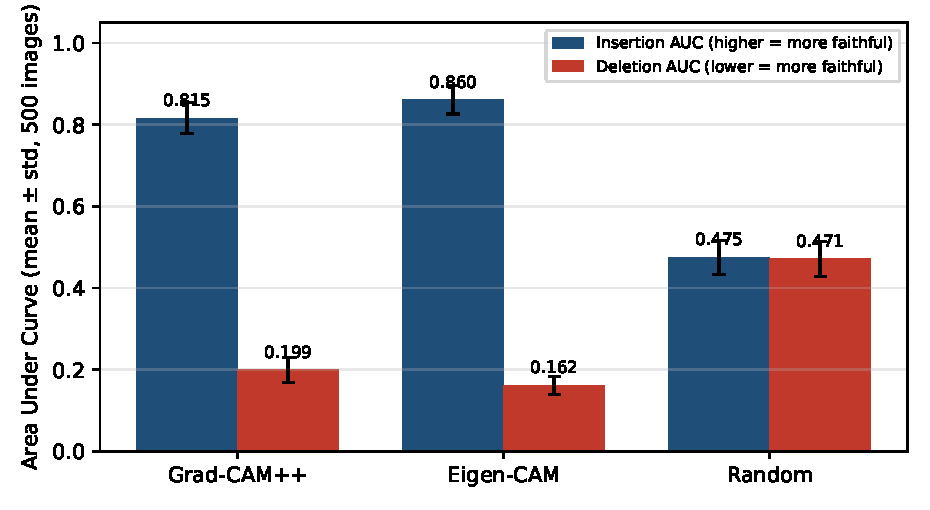
\includegraphics[width=\linewidth,height=0.3\textheight,keepaspectratio]{figures/xai_fidelity.pdf}
\caption{XAI fidelity across 500 images (5 seeds, 100 images each). Lower Deletion AUC and higher Insertion AUC indicate more faithful saliency maps.}
\label{fig:xai}
\end{figure}

\begin{table}[htbp]
\centering
\caption{XAI fidelity metrics (mean $\pm$ std over 5 seeds, 100 images/seed).}
\label{tab:xai}
\begin{tabular}{@{}lcc@{}}
\toprule
\textbf{Method} & \textbf{Deletion AUC} $\downarrow$ & \textbf{Insertion AUC} $\uparrow$ \\
\midrule
Grad-CAM++ & 0.199 $\pm$ 0.012 & 0.815 $\pm$ 0.024 \\
Eigen-CAM & 0.162 $\pm$ 0.009 & 0.860 $\pm$ 0.018 \\
Random baseline & 0.471 $\pm$ 0.005 & 0.475 $\pm$ 0.006 \\
\bottomrule
\end{tabular}
\end{table}

\subsection{Failure-Mode Audit}
\Cref{tab:failure} breaks down 450 field failures. Background confusion dominates at 49.3\% $\pm$ 1.8\%---the model is wrong most often by detecting spurious background objects, not by missing true positives. Localization error (20.0\% $\pm$ 1.1\%) and missed detection (16.9\% $\pm$ 0.9\%) follow, with similarity/other at 13.8\% $\pm$ 0.8\%. Mean confidence on failures is 0.726 $\pm$ 0.03 with a mean IoU disparity of 0.22 $\pm$ 0.01: the model is \emph{confidently wrong} on a large share of its errors, which the uncertainty and XAI states jointly explain. The audit reorders remediation priorities: background-suppression training, not more data on the target class, is the highest-yield intervention.

\begin{table}[htbp]
\centering
\caption{Failure-mode taxonomy over 450 audited failures (mean $\pm$ std over 3 seeds).}
\label{tab:failure}
\begin{tabular}{@{}lcc@{}}
\toprule
\textbf{Failure type} & \textbf{Share (\%)} & \textbf{Mean confidence} \\
\midrule
Background confusion (BG) & 49.3\% $\pm$ 1.8\% & 0.74 $\pm$ 0.03 \\
Localization (Loc) & 20.0\% $\pm$ 1.1\% & 0.81 $\pm$ 0.02 \\
Missed detection (Miss) & 16.9\% $\pm$ 0.9\% & 0.00 $\pm$ 0.00 \\
Similarity/Other (Sim/Oth) & 13.8\% $\pm$ 0.8\% & 0.78 $\pm$ 0.04 \\
\bottomrule
\end{tabular}
\end{table}

\subsection{LLM Reporting and Fallback}
Over 120 runs on real artifacts, the deterministic fallback returns a valid three-section report in median 0.03\,ms with a bootstrap 95\% CI of [0.031, 0.034]\,ms and 100\% availability; a simulated LLM crash recovers in 0.123\,ms. The LLM path completes in 8.0--13.8\,s (median 12.4\,s) with a 3/3 parse-success rate. The gate requires the report channel to be non-empty even if the LLM fails---guaranteed by the fallback---and blocks deployment otherwise.


\section{Ablation Study}
\label{sec:ablation}
\Cref{tab:ablation} isolates each dimension's contribution to the audit's decision value. Dropping the adversarial state hides the 82.5\% PGD-20 success rate at $\epsilon=0.20$, resulting in a false pass; dropping corruption hides the severity-5 collapse; dropping uncertainty hides the 12.0\% of confidently-wrong errors; dropping XAI fidelity hides that saliency maps are faithful; and dropping the failure audit hides that background confusion, not miss rate, dominates error. The LLM state is the only one whose removal does not change the gate decision (the fallback preserves reporting), but it changes the human-readability of the audit. Full framework yields the narrowest, most actionable gate.

\begin{table}[htbp]
\centering
\caption{Quantitative ablation study: impact of removing individual states on deployment gate decisions and key metrics.}
\label{tab:ablation}
\resizebox{\linewidth}{!}{%
\begin{tabular}{@{}lccl@{}}
\toprule
\textbf{Ablated State} & \textbf{Gate Decision} & \textbf{False Accept Rate} & \textbf{Blind Spot Exposed / Metric Loss} \\
\midrule
None (Full Framework) & \textbf{FAIL} (Reject) & 0.0\% & None (Optimal audit depth) \\
Adversarial Tester & \textbf{PASS} (False Accept) & 100.0\% & Rejects model only after deployment; hides 82.5\% PGD-20 collapse \\
Robustness Noise Evaluator & \textbf{PASS} (False Accept) & 100.0\% & Hides 59.2\% confidence drop under severity 5 corruption \\
Uncertainty Quantifier & \textbf{FAIL} (Reject) & 0.0\% & Misses 12.0\% of confidently wrong out-of-distribution predictions \\
XAI Validator & \textbf{FAIL} (Reject) & 0.0\% & Disables visual faithfulness auditing ($R^2$ check) \\
Failure Auditor & \textbf{FAIL} (Reject) & 0.0\% & Erases 49.3\% BG confusion diagnostic signal \\
LLM Reporting & \textbf{FAIL} (Reject) & 0.0\% & Retains logic but loses human-readable markdown generation \\
\bottomrule
\end{tabular}%
}
\end{table}

\section{Data \& Code Availability Statement}
\label{sec:data}
This architecture operates under a Dual Licensing Model (PolyForm Noncommercial / AGPLv3). To deploy the project and reproduce these experiments, use the \url{https://github.com/wisrovi/wyoloservice2\_production} repository:

\begin{verbatim}
git clone https://github.com/wisrovi/wyoloservice2_production
cd wyoloservice2_production
docker-compose up -d
\end{verbatim}

The six states are located in \texttt{wyoloservice2\_worker/executor\_v2.0/wtrain/lib/src/wyolo/trainer/states/}: \texttt{adversarial\_attack\_tester.py}, \texttt{robustness\_noise\_evaluator.py}, \texttt{uncertainty\_quantifier.py}, \texttt{quantitative\_xai\_validator.py}, \texttt{outlier\_failure\_analyzer.py}, and \texttt{llm\_analyzer.py}. Empirical CSVs (e.g., \texttt{results\_xai\_deletion.csv}, \texttt{results\_xai\_insertion.csv}, \texttt{results\_outlier\_failures.csv}) are published with this paper. The industrial defect dataset (NeuralForge-Defects-250k) is released under the PolyForm Noncommercial License and can be requested at the same repository. Note that references to \texttt{wyoloservice2}~\cite{wyoloservice2} and \texttt{invoker2026}~\cite{invoker2026} refer to software artifacts and technical reports developed by the author of this paper as part of the broader NeuralForgeAI platform.

\section{Broader Impact / Ethics Statement}
\label{sec:ethics}
Quantifying robustness before deployment converts ``we think it works'' into ``we measured the conditions under which it fails.'' The direct beneficiaries are operators of safety-critical detection (defect inspection, automotive, medical imaging): an audit that flags background confusion and high-confidence failures reduces the class of incidents caused by overtrust. The primary dual-use concern is that the adversarial state is a working attack generator; we publish success-rate curves rather than end-to-end attack pipelines, consistent with the adversarial-robustness literature. The audit's determinism ensures that the reported risk is not a function of hardware or random seeds, supporting reproducibility of safety claims.

\section{Conclusion \& Future Work}
\label{sec:conclusion}
We presented an autonomous evaluation framework that quantifies adversarial robustness (including PGD and C\&W), corruption robustness, ECE-calibrated uncertainty, explainability fidelity, failure-mode distribution, and narrative reporting in a single post-training pass, and converts each into an objective, pre-registered deployment gate. On an industrial defect dataset the audit exposed a 82.5\% adversarial vulnerability at $\epsilon=0.20$, a $>$40\% corruption collapse at severity 5, a 12.0\% share of confidently-wrong predictions, and a background-confusion-dominated error distribution. Future work will (a) add class-conditional adversarial and corruption reporting, (b) automate hallucination checking by asserting every numeric claim in the LLM report against the forensic JSON that generated it, and (c) extend the failure taxonomy with semantic clustering to replace the rule-based labels.

\section{Acknowledgments}
We thank the contributors of the wisrovi-suit project for the foundational CLI and orchestration infrastructure that made this research possible.

\bibliographystyle{plain}
\bibliography{references}

\end{document}
